% loading packages
\documentclass[a4paper,11pt]{article}
\usepackage[utf8]{inputenc} 
\usepackage[T1]{fontenc}
\usepackage{lmodern}
\usepackage[ngerman]{babel}
\usepackage{graphicx}
\usepackage{apacite}
\usepackage[document]{ragged2e}
\usepackage{enumitem}
\usepackage{acronym}
\usepackage{scrpage2}
\usepackage{array}
\pagestyle{scrheadings}
\usepackage{wasysym}
\clearscrheadfoot

\cfoot{\pagemark}

% set the formation
\setlength{\parindent}{0mm} % Neuer Absatz nichteingerückt, sonder Abstand von 1mm
\setlength{\parskip}{1mm} % Neuer Absatz nichteingerückt, sonder Abstand von 1mm

\newenvironment{conditions}
  {\par\vspace{\abovedisplayskip}\noindent\begin{tabular}{>{$}l<{$} @{${}={}$} l}}
  {\end{tabular}\par\vspace{\belowdisplayskip}}

% document
\begin{document}
\pagenumbering{gobble}  % No Pagenumbers
\newpage
\centering

\includegraphics[width=0.15\textwidth]{../images/tu_Logo/TU_Logo_kurz_1c_schwarz.pdf}\par\vspace{1cm}
{\scshape\LARGE Technische Universität Berlin\par}
\vspace{0cm}
{\scshape\normalsize Fachgebiet Bahnbetrieb und Infrastruktur\par}
\vspace{1cm}
{\scshape\LARGE Bachelorarbeit\par}
\vspace{1.5cm}
{\LARGE\bfseries Realitätsnahe Fahrzeugsteuerung\\für die Eisenbahnbetriebssimulation\\im Eisenbahn-Betriebs- und Experimentierfeld\par}
\vspace{2cm}
{\Large\itshape Friedrich Kasper Völkers\par}
\vspace{0cm}
{\normalsize 391529\par}
\vfill
betreut von\par
Dr.-Ing. Christian \textsc{Blome}
\vfill
{\large Berlin, \today\par}
\justifying
\newpage
\section*{Zusammenfassung}
Im Rahmen dieser Arbeit wurde eine Fahrzeugsteuerung entwickelt, welche die Fahrzeuge im eingleisigen Netz des \acfp{ebuef} ansteuert. Dazu wurde ein allgemeingültiger Algorithmus entwickelt, der einen möglichst optimalen \Gls{fahrtverlauf} ermittelt. Die Berechnung des \Gls{fahrtverlauf}s basiert auf den gegebenen \aclp{infra}n inklusive deren Länge und zulässiger Höchstgeschwindigkeit, der aktuellen Position und Geschwindigkeit, der Zielposition und der Ankunftszeit. Durch den ermittelten \Gls{fahrtverlauf} ist eine kontinuierliche Fahrzeugüberwachung möglich und die aktuelle Position der Fahrzeuge ist zu jedem Zeitpunkt bekannt.
\vspace{3cm}


\noindent Todo-Liste (Beim Korrekturlesen bitte nicht beachten...)
\begin{itemize}
\item Was funktioniert nicht
\item Formeln?!
\item linebreak
\item glossaries
\item acronyms
\item leerzeichen zwischen zahl und einheit
\item doppelte leerzeichen
\item \textit{\$allTrains} beschreiben
\end{itemize}
\pagenumbering{Roman} % roman pagenumbers
\tableofcontents % set the table of contents
\newpage % set new page
\listoffigures % set the table of figures
\listoftables % set the table of tables
\newpage
\begin{acronym}[Infra-Abschnitt]
\acro{ebuef}[EBuEf]{Eisenbahn-Betriebs- und Experimentierfeld}
\acroplural{ebuef}[EBuEfs]{Eisenbahn-Betriebs- und Experimentierfelds}
\acro{infra}[Infra-Ab\-""schnitt]{Infra\-struk\-tur\-ab\-schnitt}
\acrodefplural{infra}[Infra-""Ab\-schnitte]{Infra\-struk\-tur\-ab\-schnitte}
\end{acronym}
\newpage
\pagenumbering{arabic} % arabic pagenumbers
\section{Grundlagen}

\subsection{Zitate}

At vero eos et accusam et justo duo dolores et ea rebum. Stet clita kasd gubergren, no sea takimata sanctus est Lorem ipsum dolor sit amet. Duis autem vel eum iriure dolor in hendrerit in vulputate velit esse molestie consequat, vel illum dolore eu feugiat nulla facilisis at vero eros et accumsan et iusto odio dignissim qui blandit praesent luptatum zzril delenit augue duis dolore te feugait nulla facilisi. Lorem ipsum dolor sit amet.

Lorem ipsum dolor sit amet, consetetur sadipscing elitr, sasd gubergren, no sea takimata sanctus est Lorem ipsum dolor sit amet. L consequat, vel illum dolore eu feugiat nulla facilisis at vero eros et accumsan et iusto odio dignissim qui blandit praesent luptatum zzril delenit augue duis dolore te feugait nulla facilisi. Lorem ipsum dolor sit amet.\cite{maschek2013zugbeeinflussung}, \cite{wende2013fahrdynamik} Lorem ipsum dolor sit amem nonumore et dolore magna aliquyam erat, sed diam voluptua. At vero eos et accusam et justo duo dolores et ea rebum. Stet clita kasd gubimata sanctus est Lorem ipsum dolor sit amet. Lorem ipsum dolor sit amet, consetetur sadipscing elitr, sed diam nonumgnoluptua. At vero eos lor sit amet. Loreonumy eirmod tempor invidunt ut labore et dolore magna aliquyam clita kasd gubergren, no sea takimata sanctus est Lorem ipsum dolor sit amet. Duis autem vel eum iriure dolor in hendrerit in vulputate velit esse molestie consequat, vel illum dolore eu feugiat nulla facilisis at vero eros et accumsan et iusto odio dignissim qui blandit praesent luptatum zzril delenit augue duis dolore te feugait nulla facilisi. Lorem ipsum dolor sit amet.\cite{maschek2013zugbeeinflussung}, \cite{wende2013fahrdynamik}

\subsection{Abkürzungen}

Lorem ipsum dolor sit amet, consetetur sadipscing elitr, sed diam nonumy eirmod tempor invidunt ut labore et dolore magna aliquyam erat, sed diam voluptua. At vero eos et accusam et justo duo dolores et ea rebum. Stet clita kasd gubergren, no sea takimata  sanctus est Lorem ipsum dolor sit amet. Lorem ipsum dolor sit amet, consetetur sadipscing elitr, \ac{re} sed diam nonumy eirmod tempor invidunt ut labore et dolore magna aliquyam erat, sed diam voluptua. At vero eos et accusam et justo duo dolores et ea rebum. Stet clita kasd gubergren, no sea takimata sanctus est Lorem ipsum dolor sit amet. Lorem ipsum dolor sit amet, consetetur sadipscing elitr, sed diam nonumy eirmod tempor invidunt ut labore et \ac{ice} dolore magna aliquyam erat, sed diam  \ac{pz} voluptua. At vero eos et accusam et justo duo dolores et ea rebum. Stet clita kasd gubergren, no sea takimata sanctus est Lorem ipsum dolor sit amet. Duis autem vel eum iriure dolor in hendrerit in vulputate velit esse molestie consequat, vel illum dolore eu feugiat nulla facilisis at vero eros et accumsan et iusto odio dignissim qui blandit praesent luptatum zzril delenit augue duis dolore te feugait nulla facilisi. Lorem ipsum dolor sit amet \ac{pz}.

\subsection{Zitat}

\begin{quote}
\label{intro}„Hongkong must build a [...] rapid transit system, or a more expensive roads system, in the next 16 years – or face potentially devastating effects on its economy.“
\end{quote}

\subsection{Bild}

\begin{figure}[h]
  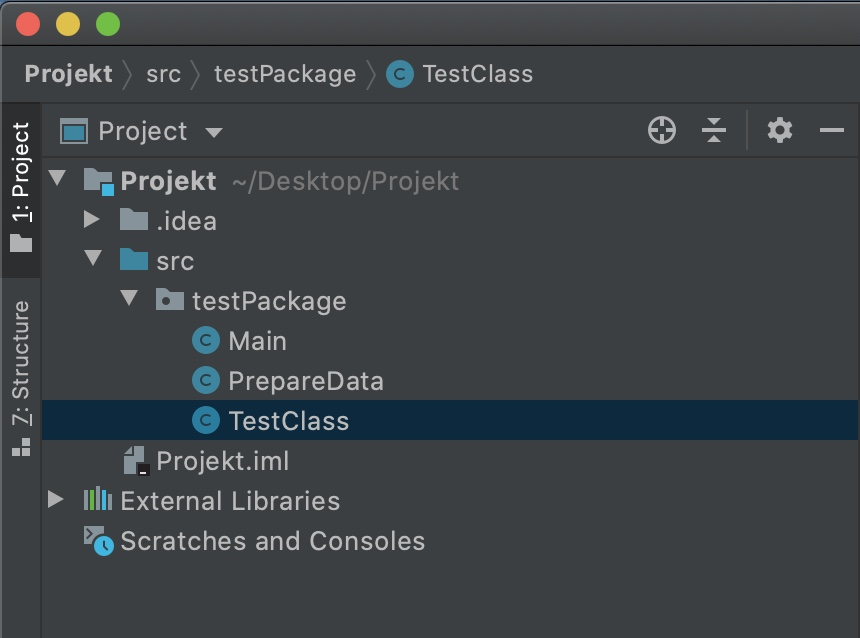
\includegraphics[width=\linewidth]{Images/img1.jpg}
  \caption{Darstellung eines Bahnhofs}
\end{figure}

\subsection{Tabelle}

\begin{table}[h]
\begin{center}
\begin{tabular}[h]{c|c|c}
ICE 1 & ICE 2 & ICE 3 \\ \hline
200 km/h & 250 km/h  & 300 km/h  \\
\end{tabular}
\caption{Sehr sehr schöne Tabelle}
\end{center}
\end{table} % implement chapter .tex file from the same folder
\newpage
\section{Formeln} \label{formula}
\begin{flushleft}
Für die im folgenden Kapitel verwendeten Einheiten gilt:
\end{flushleft}

\begin{centering}
\begin{conditions}
a     &  Bremsverzoegerung [$m/s^{2}$] \\
v     &  Geschwindigkeit [$m/s$] \\
s     &  Strecke [$m$] \\
t     &  Zeit [$s$]
\end{conditions}
\end{centering}
\subsection{Formeln für gleichmäßig beschleunigte Bewegungen} \label{formulaBeschleunigung}
\noindent Bei einer gleichmäßig beschleunigten Bewegung gilt:\footnote{\citet[S. 22]{richard2011technische}}
\begin{equation}
a(t) = a
\end{equation}
Für die Bestimmung der Geschwindigkeit in Abhängigkeit der Zeit, muss die Beschleunigung $a(t)$ nach der Zeit $t$ integriert werden.\footnote{\citet[S. 20]{richard2011technische}}
\begin{equation}
v(t) = \int a(t) \,dt
\end{equation}
Daraus ergibt sich folgende Gleichung für die Geschwindigkeit in Abhängigkeit der Zeit. Die bei der Integration entstehende Integrationskonstante $v_{0}$ gibt dabei die Startgeschwindigkeit an.
\begin{equation}
v(t) = a \cdot t + v_{0}
\end{equation} %\footnote{ebd. (S. 20)}
Für die Bestimmung der benötigten Zeit muss die Geschwindigkeit erneut integriert werden.\footnote{\citet[S. 20]{richard2011technische}} Die dabei entstehende Integrationskonstante $s_{0}$ gibt die bereits zurückgelegte Strecke an.
\begin{equation}
s(t) = \int v(t) \,dt
\end{equation}
\begin{equation}
s(t) =\frac{1}{2} \cdot a \cdot t^{2} + v_{0}  \cdot t + s_{0}
\end{equation}
Bei der Verwendung dieser Gleichung werden die Integrationskonstanten $v_{0}$ und $s_{0}$ gleich $0$ gesetzt, damit die Gleichungen allgemein gültig sind. Für die Berechnung des Beschleuniguns- und Abbremsverhalten der Fahrzeuge ist es notwendig zu wissen, welche Strecke ein Fahrzeug zurücklegen muss, um von einer Startgeschwindigkeit $v_{0}$ auf eine Zielgeschwindigkeit $v_{1}$ zu beschleunigen bzw. abzubremsen. Dafür wird die Gleichung für die Geschwindigkeit $v(t)$ nach $t(v)$ umgestellt und und in die Gleichung $s(t)$ eingesetzt. Daraus ergibt sich folgende Gleichung für die Strecke in Abhängigkeit von der Geschwindigkeit:
\begin{equation}
t(v) = \frac{v}{a}
\end{equation}
\begin{equation}
s(v) =\frac{1}{2} \cdot \frac{v^{2}}{a}
\end{equation}
Durch die Festlegung von $v_{0} = 0$ wird so die benötigte Strecke ermittelt, welche ein Fahrzeug bei einer gegebenen Bremsverzögerung $a$ benötigt, um von 0 $m/s$ auf eine gegebenen Zielgeschwindigkeit $v_{1}$ zu beschleunigen. Bei der Berechnung des Beschleuniguns- und Abbremsverhalten wird es aber auch zu Situationen kommen, bei denen ein Fahrzeug eine Startgeschwindigkeit hat, für die gilt $v_{0} \neq 0$. Um eine allgemein gültige Gleichung aufzustellen, wird für die Ermittlung der benötigten Strecke bei einer gegebenen Start- und Zielgeschwindigkeit die Strecke berechnet, die das Fahrzeug benötigt, um von 0 $m/s$ auf $v_{1}$ und von 0 $m/s$ auf $v_{0}$ zu beschleunigen. Für die gesuchte Strecke gilt dann: 
\begin{equation}
s(v_{0}, v_{1}) = \abs{s(v_{1}) - s(v_{0})} 
\end{equation}
\begin{equation}
\label{eq:s_v_ges}
s(v_{0}, v_{1}) =\frac{1}{2} \cdot\abs{\frac{v_{1}^{2} - v_{0}^{2}}{a}}
\end{equation}
In der Fahrzeugsteuerung übernimmt diese Berechnung die Funktion \textit{getBrakeDistance()} (Code-Beispiel \ref{lst:getBrakeDistance}). 
\begin{figure}[H]
\begin{lstlisting}[caption={\textit{getBrakeDistance$($$)$} (\textit{functions\_math.php})},captionpos=b,label={lst:getBrakeDistance}]
// Ermittlung der Strecke für eine Beschleunigung bzw. Verzögerung
function getBrakeDistance (float $v_0, float $v_1, float $verzoegerung) {
	return abs(0.5 * ((pow($v_0/3.6,2) - pow($v_1/3.6, 2))/($verzoegerung)));
}
\end{lstlisting}
\end{figure}
\noindent Neben der Berechnung der Strecke ist auch die benötigte Zeit essenziell. Dafür wird mittels $t(v)$ die Zeit berechnet, die das Fahrzeug benötigt, um von 0 $km/h$ auf $v_{0}$ bzw. $v_{1}$ zu beschleunigen und aus der Differenz wird die benötigte Zeit berechnet.
\begin{equation}
\label{eq:t_v_ges}
t(v_{0}, v_{1}) = \abs{\frac{v_{1} - v_{0}}{a}}
\end{equation}
In der Fahrzeugsteuerung übernimmt diese Berechnung die Funktion \textit{getBrakeTime()} (\textit{func\-tions\_""math\-.php}) (Code-Beispiel \ref{lst:getBrakeTime}).
\begin{figure}[H]
\begin{lstlisting}[caption={\textit{getBrakeTime$($$)$} (\textit{functions\_math.php})},captionpos=b,label={lst:getBrakeTime}]
// Ermittelt die Distanz für Brems- und Verzögerungsvorgänge
function getBrakeTime (float $v_0, float $v_1, float $verzoegerung) {
	return abs((($v_1/3.6)/$verzoegerung) - (($v_0/3.6)/$verzoegerung));
}
\end{lstlisting}
\end{figure}
\noindent Für die Berechnung einer Gefahrenbremsung ist es notwendig zu wissen, welche Geschwindigkeit das Fahrzeug an der Position der Gefahrenstelle hat. Dafür wird die Gleichung \eqref{eq:s_v_ges} nach $v_{2}$ umgestellt. Umgesetzt wird diese Gleichung mit der Funktion \textit{get\-Tar\-get\-Brake\-Speed\-With\-Dis\-tance\-And\-Start\-Speed$($$)$} (\textit{func\-tions\_""math\-.php}) (Code-Beispiel \ref{lst:getTargetBrakeSpeedWithDistanceAndStartSpeed}).
\begin{equation}
\label{eq:gefahrenbremsung}
v_{2}(v_{1}, s) = \sqrt{-2 \cdot s \cdot a} + v_{1}
\end{equation}
\begin{figure}[H]
\begin{lstlisting}[caption={\textit{getTargetBrakeSpeedWithDistanceAndStartSpeed$($$)$} (\textit{func\-tions\_""math\-.php})},captionpos=b,label={lst:getTargetBrakeSpeedWithDistanceAndStartSpeed}]
// Ermittelt die Geschwindigkeit, die ein Fahrzeug in einem Bremsvorgang
// nach einer gegebenen Distanz hat.
function getTargetBrakeSpeedWithDistanceAndStartSpeed (float $distance, float $verzoegerung, int $speed) {
	return sqrt((-2 * $verzoegerung * $distance) + (pow(($speed / 3.6), 2)))*3.6;
}
\end{lstlisting}
\end{figure}
\subsection{Formeln für gleichförmige Bewegungen} \label{formulaGleichfoermig}
Bei einer gleichförmigen Bewegung gilt der Grundsatz:\footnote{\citet[S. 22]{richard2011technische}}
\begin{equation}
v(t) = v
\end{equation}
Für die Berechnung der Strecke gilt wie bei der gleichmäßig beschleunigten Bewegung:\footnote{\citet[S. 20]{richard2011technische}}
\begin{equation}
s(t) = \int v(t) \,dt
\end{equation}
\begin{equation}
s(t) =v \cdot t + s_{0}
\end{equation}
Damit die Gleichung allgemeingültig ist, wird die Integrationskonstante $s_{0}$ gleich 0 gesetzt.
\begin{equation}
s(t) =v \cdot t
\label{eq:s_v_t}
\end{equation}
\begin{figure}[H]
\begin{lstlisting}[caption={\textit{distanceWithSpeedToTime$($$)$} (\textit{functions\_math.php})},captionpos=b,label={lst:distanceWithSpeedToTime}]
// Ermittelt die Zeit, die ein Fahrzeug bei einer gegebenen Strecke für
// eine gegebene Distanz benötigt
function distanceWithSpeedToTime (int $v, float $distance) {
	return (($distance)/($v / 3.6));
}
\end{lstlisting}
\end{figure}
\noindent Für die Einhaltung der exakten Ankunftszeit, muss errechnet werden, wie lange das Fahrzeug bei zwei gegebenen Geschwindigkeiten ($v_1$ und $v_2$) auf den jeweiligen Geschwindigkeiten fahren muss, um die Gesamtstrecke ($s_{ges}$) und die Gesamtzeit ($t_{ges}$) einzuhalten. Für die Zeiten und Strecken gilt:
\begin{equation}
\label{eq:t_ges}
t_{ges} = t_{1} + t_{2}
\end{equation}
\begin{equation}
\label{eq:s_ges}
s_{ges} = s_{1} + s_{2}
\end{equation}
Durch das Einsetzen der Gleichung \eqref{eq:s_v_t} in die Gleichung \eqref{eq:s_ges} erhält man folgende Gleichung:
\begin{equation}
\label{eq:s_ges_2}
s_{ges} = v_{1} \cdot t_{1} + v_{2} \cdot t_{2}
\end{equation}
Durch das Umstellen der Gleichung \eqref{eq:t_ges} nach $t_{2}$ und dem Einsetzen in Gleichung \eqref{eq:s_ges_2} gilt für $t_{1}$:
\begin{equation}
\label{eq:t_1_tuning}
t_{1} = \frac{s_{ges} - v_{2} \cdot t_{ges}}{v_{1} - v_{2}}
\end{equation}
\begin{figure}[H]
\begin{lstlisting}[caption={\textit{calculateDistanceforSpeedFineTuning$($$)$} (\textit{functions\_math.php})},captionpos=b,label={lst:calculateDistanceforSpeedFineTuning}]
// Ermittelt die Distanz, um die eine Verzögerung "verschoben" werden müsste,
// damit die exakte Ankunftszeit eingehalten werden kann.
function calculateDistanceforSpeedFineTuning(int $v_0, int $v_1, float $distance, float $time) : float {
	return $distance - (($distance - $time * $v_1 / 3.6)/($v_0 / 3.6 - $v_1 / 3.6)) * ($v_0 / 3.6);
}
\end{lstlisting}
\end{figure}
\newpage
\pagenumbering{Roman} % roman pagenumbers
\setcounter{page}{4}
\bibliographystyle{apacite} % set the referencepage
\bibliography{paper}  % implement the name of the bibtex.bib file
\end{document}